\documentclass{standalone}
\usepackage{tikz}
\usetikzlibrary{automata, positioning, arrows.meta, arrows}

\begin{document}
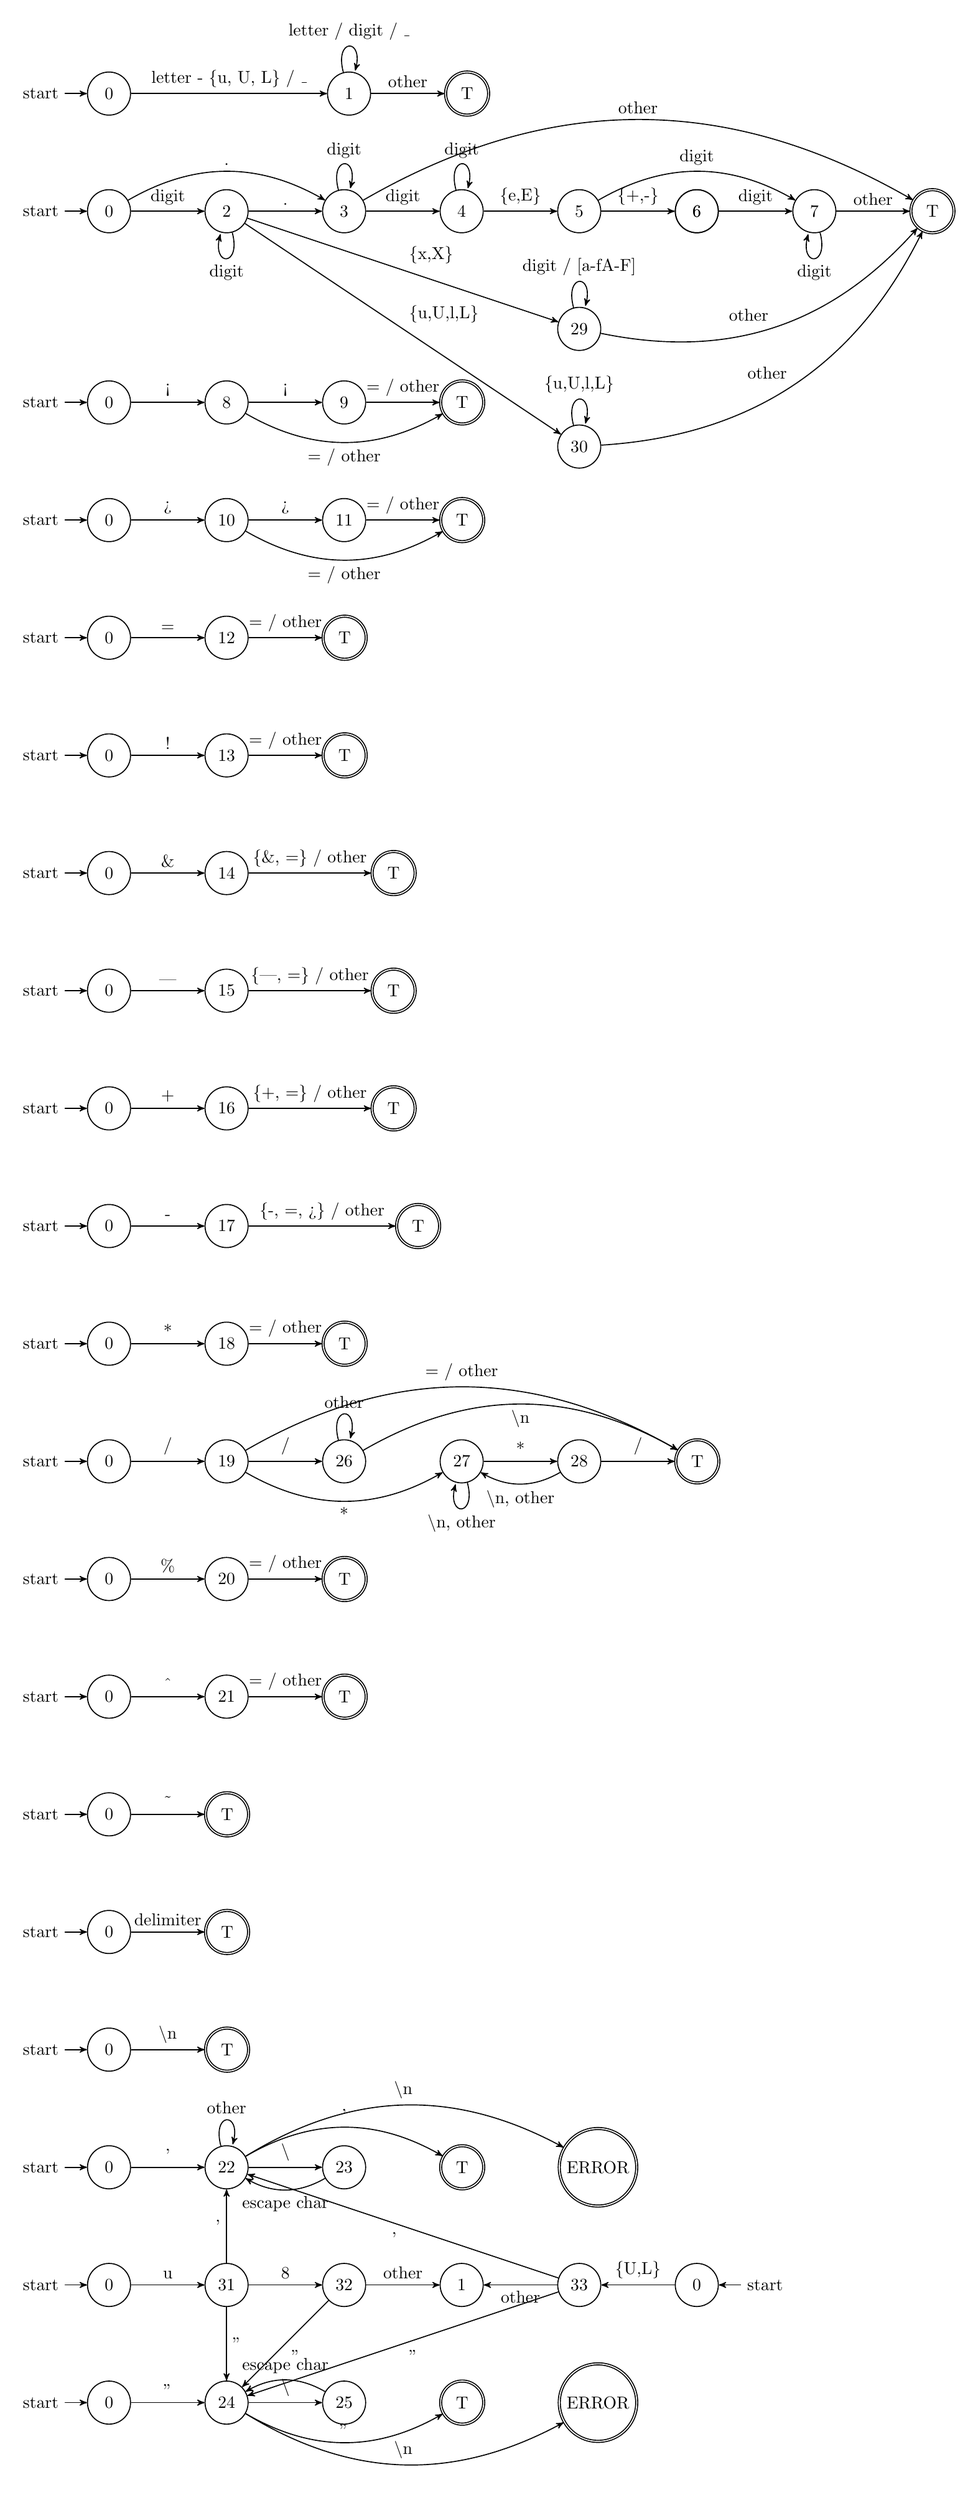
\begin{tikzpicture}[->, >=stealth', auto, node distance=1.5cm, semithick, transform shape]
    \node[state, initial] (q00) {0};
    \node[state] (q1) [right=of q00, xshift=2.5cm] {1};
    \node[state, accepting] (t0) [right=of q1] {T};
    \path
    (q00) edge node {letter - \{u, U, L\} / \_} (q1)
    (q1) edge [loop above] node {letter / digit / \_} (q1)
    (q1) edge node {other} (t0);

    %%%%

    \node[state, initial] (q01) [below=of q00] {0};
    \node[state] (q2) [right=of q01] {2};
    \node[state] (q3) [right=of q2] {3};
    \node[state] (q4) [right=of q3] {4};
    \node[state] (q5) [right=of q4] {5};
    \node[state] (q6) [right=of q5] {6};
    \node[state] (q6) [right=of q5] {6};
    \node[state] (q7) [right=of q6] {7};
    \node[state, accepting] (t1) [right=of q7] {T};
    \path
    (q01) edge node {digit} (q2)
    (q01) edge [bend left] node {.} (q3)
    (q2) edge [loop below] node {digit} (q2)
    (q2) edge node {.} (q3)
    (q3) edge [loop above] node {digit} (q3)
    (q3) edge node {digit} (q4)
    (q3) edge [bend left] node {other} (t1)
    (q4) edge [loop above] node {digit} (q4)
    (q4) edge node {\{e,E\}} (q5)
    (q5) edge node {\{+,-\}} (q6)
    (q5) edge [bend left] node [above] {digit} (q7)
    (q6) edge node {digit} (q7)
    (q7) edge [loop below] node {digit} (q7)
    (q7) edge node {other} (t1);

    \node[state] (q29) [below=of q5] {29};
    \path
    (q2) edge node {\{x,X\}} (q29)
    (q29) edge [loop above] node {digit / [a-fA-F]} (q29)
    (q29) edge [bend right] node {other} (t1);

    \node[state] (q30) [below=of q29] {30};
    \path
    (q2) edge node {\{u,U,l,L\}} (q30)
    (q30) edge [loop above] node {\{u,U,l,L\}} (q30)
    (q30) edge [bend right] node {other} (t1);
    
    %%%

    \node[state, initial] (q02) [below=of q01, yshift=-1.5cm] {0};
    \node[state] (q8) [right=of q02] {8}; % to T
    \node[state] (q9) [right=of q8] {9};
    \node[state, accepting] (t2) [right=of q9] {T};
    \path
    (q02) edge node {<} (q8)
    (q8) edge [bend right] node [below] {= / other} (t2)
    (q8) edge node {<} (q9)
    (q9) edge node {= / other} (t2);

    %%%

    \node[state, initial] (q03) [below=of q02] {0};
    \node[state] (q10) [right=of q03] {10}; % to T
    \node[state] (q11) [right=of q10] {11};
    \node[state, accepting] (t3) [right=of q11] {T};
    \path
    (q03) edge node {>} (q10)
    (q10) edge [bend right] node [below] {= / other} (t3)
    (q10) edge node {>} (q11)
    (q11) edge node {= / other} (t3);

    %%%

    \node[state, initial] (q04) [below=of q03] {0};
    \node[state] (q12) [right=of q04] {12};
    \node[state, accepting] (t4) [right=of q12] {T};
    \path
    (q04) edge node {=} (q12)
    (q12) edge node {= / other} (t4);

    %%%

    \node[state, initial] (q05) [below=of q04] {0};
    \node[state] (q13) [right=of q05] {13};
    \node[state, accepting] (t5) [right=of q13] {T};
    \path
    (q05) edge node {!} (q13)
    (q13) edge node {= / other} (t5);

    %%%

    \node[state, initial] (q06) [below=of q05] {0};
    \node[state] (q14) [right=of q06] {14};
    \node[state, accepting] (t6) [right=of q14, xshift=1cm] {T};
    \path
    (q06) edge node {\&} (q14)
    (q14) edge node {\{\&, =\} / other} (t6);

    %%%

    \node[state, initial] (q07) [below=of q06] {0};
    \node[state] (q15) [right=of q07] {15};
    \node[state, accepting] (t7) [right=of q15, xshift=1cm] {T};
    \path
    (q07) edge node {|} (q15)
    (q15) edge node {\{|, =\} / other} (t7);

    %%%

    \node[state, initial] (q08) [below=of q07] {0};
    \node[state] (q16) [right=of q08] {16};
    \node[state, accepting] (t8) [right=of q16, xshift=1cm] {T};
    \path
    (q08) edge node {+} (q16)
    (q16) edge node {\{+, =\} / other} (t8);

    %%%

    \node[state, initial] (q09) [below=of q08] {0};
    \node[state] (q17) [right=of q09] {17};
    \node[state, accepting] (t9) [right=of q17, xshift=1.5cm] {T};
    \path
    (q09) edge node {-} (q17)
    (q17) edge node {\{-, =, >\} / other} (t9);

    %%%

    \node[state, initial] (q010) [below=of q09] {0};
    \node[state] (q18) [right=of q010] {18};
    \node[state, accepting] (t10) [right=of q18] {T};
    \path
    (q010) edge node {*} (q18)
    (q18) edge node {= / other} (t10);

    %%%

    \node[state, initial] (q011) [below=of q010] {0};
    \node[state] (q19) [right=of q011] {19};
    \node[state] (q26) [right=of q19] {26}; 
    \node[state] (q27) [right=of q26] {27};
    \node[state] (q28) [right=of q27] {28};
    \node[state, accepting] (t11) [right=of q28] {T};
    \path
    (q011) edge node {/} (q19)
    (q19) edge [bend left] node {= / other} (t11)
    (q19) edge node {/} (q26)
    (q19) edge [bend right] node [below] {*} (q27)
    (q26) edge [bend left] node [below] {\textbackslash n} (t11)
    (q26) edge [loop above] node {other} (q26)
    (q27) edge node {*} (q28)
    (q27) edge [loop below] node {\textbackslash n, other} (q27)
    (q28) edge node {/} (t11)
    (q28) edge [bend left] node [below] {\textbackslash n, other} (q27);

    %%%

    \node[state, initial] (q012) [below=of q011] {0};
    \node[state] (q20) [right=of q012] {20};
    \node[state, accepting] (t12) [right=of q20] {T};
    \path
    (q012) edge node {\%} (q20)
    (q20) edge node {= / other} (t12);

    %%%

    \node[state, initial] (q013) [below=of q012] {0};
    \node[state] (q21) [right=of q013] {21};
    \node[state, accepting] (t13) [right=of q21] {T};
    \path
    (q013) edge node {\^{}} (q21)
    (q21) edge node {= / other} (t13);

    %%%

    \node[state, initial] (q014) [below=of q013] {0};
    \node[state, accepting] (t14) [right=of q014] {T};
    \path
    (q014) edge node {\~{}} (t14);    

    %%%

    \node[state, initial] (q015) [below=of q014] {0};
    \node[state, accepting] (t15) [right=of q015] {T};
    \path
    (q015) edge node {delimiter} (t15); 

    %%%

    \node[state, initial] (q016) [below=of q015] {0};
    \node[state, accepting] (t16) [right=of q016] {T};
    \path
    (q016) edge node {\textbackslash n} (t16); 

    %%%

    \node[state, initial] (q017) [below=of q016] {0};
    \node[state] (q22) [right=of q017] {22};
    \node[state] (q23) [right=of q22] {23};
    \node[state, accepting] (t17) [right=of q23] {T};
    \node[state, accepting] (err) [right=of t17] {ERROR};
    \path
    (q017) edge node {'} (q22)
    (q22) edge node {\textbackslash} (q23)
    (q23) edge [bend left] node [below] {escape char} (q22)
    (q22) edge [bend left] node {'} (t17)
    (q22) edge [bend left] node {\textbackslash n} (err)
    (q22) edge [loop above] node {other} (q22);

    %%%

    \node[state, initial] (q019) [below=of q017] {0};

    %%%

    \node[state, initial] (q018) [below=of q019] {0};
    \node[state] (q24) [right=of q018] {24};
    \node[state] (q25) [right=of q24] {25};
    \node[state, accepting] (t18) [right=of q25] {T};
    \node[state, accepting] (err0) [right=of t18] {ERROR};
    \path
    (q018) edge node {"} (q24)
    (q24) edge node {\textbackslash} (q25)
    (q25) edge [bend right] node [above] {escape char} (q24)
    (q24) edge [bend right] node {"} (t18)
    (q24) edge [bend right] node {\textbackslash n} (err0);

    %%%

    \node[state] (q31) [right=of q019] {31};
    \node[state] (q32) [right=of q31] {32};
    \node[state] (q1_1) [right=of q32] {1};
    
    \path
    (q019) edge node {u} (q31)
    (q31) edge node {"} (q24)
    (q31) edge node {'} (q22)
    (q31) edge node {8} (q32)
    (q32) edge node {"} (q24)
    (q32) edge node {other} (q1_1);

    %%%

    \node[state] (q33) [right=of q1_1] {33};
    \node[state, initial right] (q020) [right=of q33] {0};
    \path
    (q020) edge node [above] {\{U,L\}} (q33)
    (q33) edge node {"} (q24)
    (q33) edge node {'} (q22)
    (q33) edge node {other} (q1_1);


    
    % Adding more details can be done similarly for other states and transitions
    % Customize the graph as needed to include all states and specific transitions
    % found in the code.

\end{tikzpicture}
\end{document}